\clearpage
\section{}
Podano na linię długą falę prostokątną o częstotliwości 1Mhz i przy braku połączenia drugiego końca lini (\(R\approx\infty\)) zaobserwowano nałożenie się fali biegnącej i fali odbitej.
Pomiar powtórzono dla lini zwartej \(R\approx0\) oraz dla \(R\) dopasowanego tak aby uzyskać możliwie najmniejsze odbicia.
Zmierzono również opóźnienie czasowe powstałe na skutek różnego czasu propagacji sygnału.

Znaleziona impedancja charakterystyczna \(Z=57.3\Omega\), co odpowiada założeniu prawidłowo zwartej linii tj. impedancja źródłowa i obciążenia są sobie równe, (znamionowa impedancja wyjściowa generatora to \(50\Omega\)).
Długość linii długiej \(l=16.3m\) co dla zmierzonego czasu propagacji \(t=72\)ns daje \(v=226.4\cdot10^{6}\frac{m}{s}=0.755c\), typowy czas to \(\sim5\frac{\text{ns}}{\text{m}}\) co dla badanej linii daje \(\sim81.5\)ns, wartość zbliżoną do zmierzonej.

\begin{figure}[H]
	\centering
	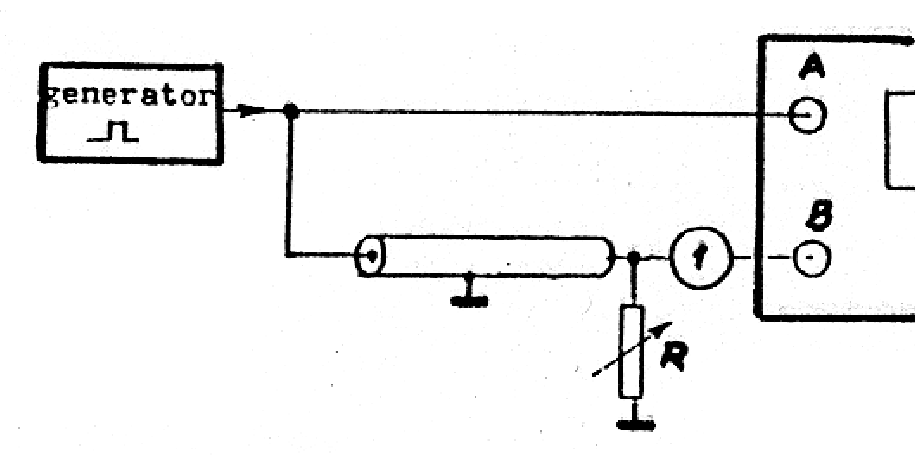
\includegraphics[width=3in]{include/5/sch.png}
	\caption{Schemat układu pomiarowego}
\end{figure}

\begin{figure}[H]
	\centering
	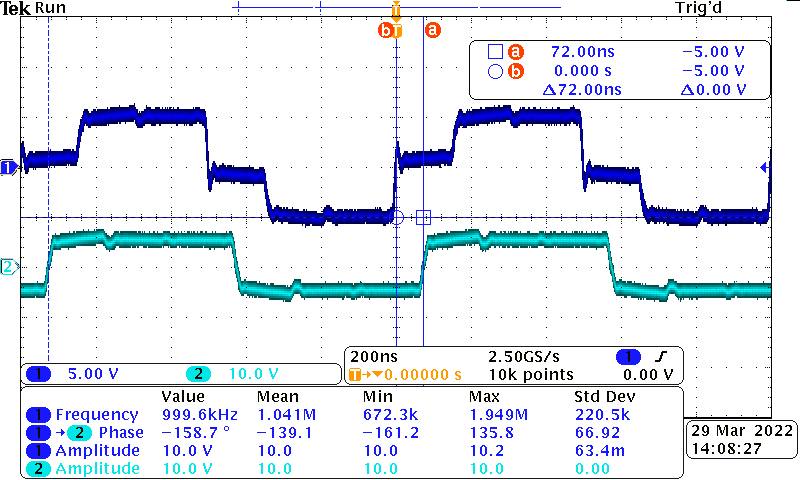
\includegraphics[width=\textwidth]{include/5/infR.png}
	\caption{Pomiar odbicia dla \(R\approx\infty\)}
\end{figure}

\begin{figure}[H]
	\centering
	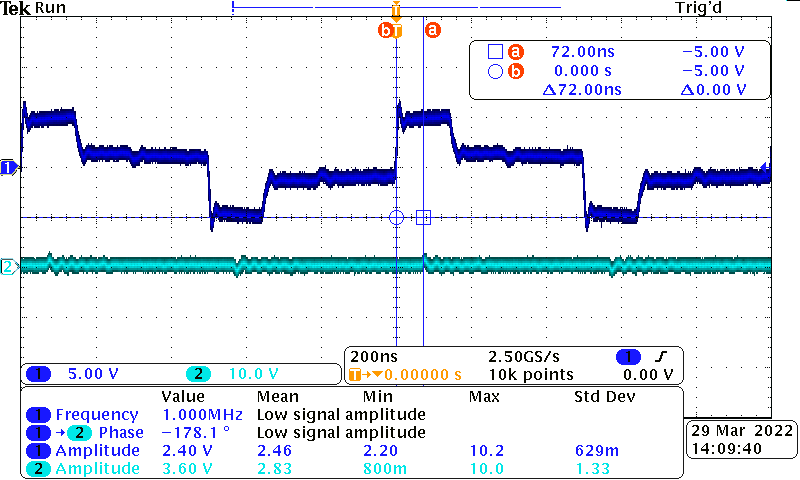
\includegraphics[width=\textwidth]{include/5/0R.png}
	\caption{Pomiar odbicia dla \(R\approx0\)}
\end{figure}

\begin{figure}[H]
	\centering
	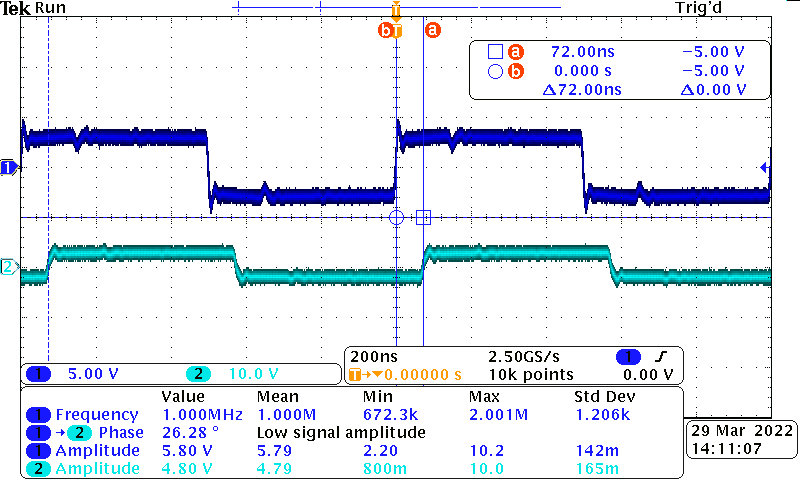
\includegraphics[width=\textwidth]{include/5/57.3R.png}
	\caption{Pomiar odbicia dla \(R=57.3\Omega\)}
\end{figure}
